\documentclass{standalone}
\usepackage{tikz, fkmath}
\begin{document}
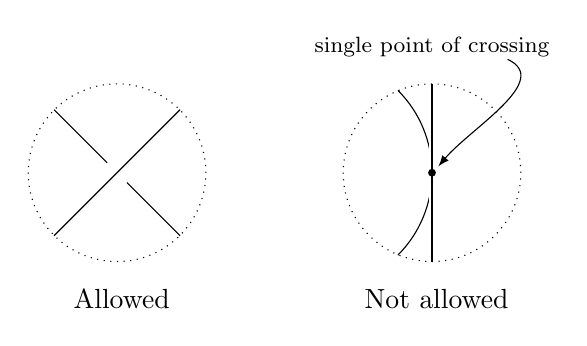
\begin{tikzpicture}[scale=.8]
  \begin{scope}[xshift=-2.5cm]
    \draw (-1,1) -- (1,-1);
    \draw[white, line width=10pt] (1,1) -- (-1,-1);
    \draw (1,1) -- (-1,-1);
    \node () at (0,-2) {\cmark\ Allowed};
    \draw[dotted] (0,0) circle (1.41);
  \end{scope}

  \begin{scope}[xshift=2.5cm]
    \draw (-.541, 1.307) to[out=-45, in=45] (-.541,-1.307);
    \draw[white, line width=2pt] (0,-1.41) -- (0,1.41);
    \draw (0,-1.41) -- (0,1.41);
    \node[circle, fill=black, inner sep=1pt] (0,0) {};
    \node () at (0,-2) {\xmark\ Not allowed};
    \node () at (0, 2) {\footnotesize single point of crossing};
    \draw[-latex] (1.2,1.8) to[out=-25, in=50] (.1,.1);
    \draw[dotted] (0,0) circle (1.41);
  \end{scope}
\end{tikzpicture}
\end{document}
